\subsection{Memory Affinity}
\label{sub:memory_affinity}

While the OpenMP~5.0 will specify task affinity based on memory locations 
as discussed in Section~\ref{sub:new_tasking}, a longer term goal is to 
support more general memory affinity. Intuitive interfaces for this complex 
problem are difficult to specify. Nonetheless, we have explored interfaces
that associate data to computation and then appropriately locate, transform 
or replicate the data based on the distribution of the computation of existing
mechanisms in OpenMP~\cite{ctsar-tpds,scogland:7Hpt64iV}.
 
Figure~\ref{fig:atsar-gemm} shows a more recent direction that specifies how
to partition computation and to map the associated data range to the threads 
of a \texttt{parallel} region and then to a set of devices. This example partitions 
the GEMM loop into two-dimensional tiles by columns across sockets and rows 
across devices associated with a given socket. Extensions like this require 
careful consideration due to their potentially large number of changes, and 
high complexity, but the information can support significant optimizations.
Beyond providing affinity information, these annotations are sufficient to 
allow for cross-device coscheduling across non-shared-memory devices.

Figure~\ref{fig:atsar-perf} shows performance results from a prototype 
implementation across five benchmark kernels in terms of speedup over a 
baseline OpenMP static schedule that uses all cores. The annotations and 
scheduling improvements that the information enables can increase performance 
substantially.  The optimization space being explored in the figure is twofold.
First is a pair of scheduling algorithms designed to be used with partitioning,
either a classic static even scheduling, and an adaptive scheduler that attempts
to predict the best partitioning based on past performance.  The CPU adaptive
results represent using the adaptive scheduler on the same resources as the
baseline.  The second axis is the set of devices the runtime system is allowed
to use when distributing computation, and data.  It can be the CPU cores only, a
set of one to four NVIDIA c1060 GPUs, or both.  All of these options can be
targeted with the same base code, in the case of GEMM the code in
Figure~\ref{fig:atsar-gemm}, just changing runtime parameters.

The amount of expressive power this kind of extension can provide is
significant, but so is the complexity and the burden on the programmer who is
trying to use it.  We intend to continue exploring this space in the future to
provide an appropriate long-term solution.

\begin{figure}
  \begin{minted}[fontsize=\footnotesize]{c}
int i, is=0, ie=isz, j, js=0, je=jsz;
float A[ksz][jsz], B[isz][ksz];
float * C = (float*)malloc(sizeof(C[0])*isz*jsz);
int   C_pitch = jsz;

#pragma omp parallel devices(socket)              \
 part(adaptive: j_id=js; j_id<je; ++j_id)         \
 map(to: A[0:ksz][:,part=j_id], B[0:isz][0:ksz])  \
 map(tofrom: C[0:isz,pitch=C_pitch][:,part=j_id])
{ // Partitioned parallel region
#pragma omp target teams distribute parallel for  \
  devices(all) partition(dynamic)                 \
  map(to: A[:][:], B[:,partition=i][:])           \
  map(tofrom: C[:,partition=i][:])
  for (int i = is; i < ie; ++i) {//Partitioned loop
    for (int j = js; j < je; ++j) {
      float sum = 0.0;
      for (int k = 0; k < ksz; ++k) {
        sum += A[k][j] * B[i][k];
      }
      C[i * C_pitch + j] = sum;
    }
  }
}
\end{minted}
\caption{Possible Memory Affinity Interface\label{fig:atsar-gemm}}
\end{figure}

\begin{figure*}[t]
        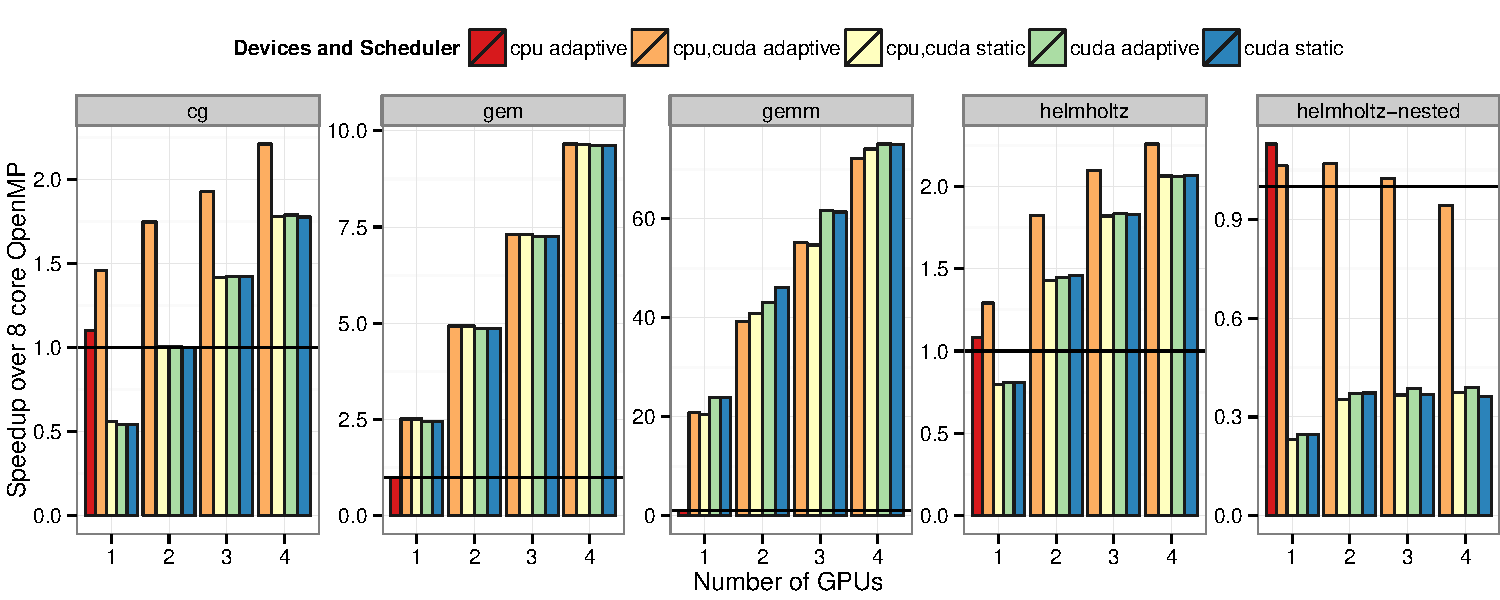
\includegraphics[width=\textwidth]{system-1-combined-part}
        \caption{Performance Benefit of Memory Partitioning/Affinity\label{fig:atsar-perf}}
\end{figure*}


